\section{Monte Carlo Methods}\label{sec:Monte_Carlo}

While they alleviate, to a degree, the limitations induced by \eqref{eq:Kalman_assumptions}, Kalman-based methods all rely on the assumption that the PDF admits a Gaussian closed-form expression at each time step. This assumption is often violated in practice, as navigation problems frequently involve highly non-linear and non-injective functions. In turn, these functions induce multimodal or heavy-tailed distributions which cannot be adequately characterised by Gaussian hypotheses.

Monte Carlo (MC) methods offer an alternative approach that is asymptotically optimal under very weak assumptions, at the cost of higher computational cost. This section introduces the main concepts for MC-based algorithms to solve the navigation problem \eqref{eq:navigation_problem}.

\subsection{Monte Carlo Integration}

Let $X$ be a random variable taking values in $\mathbb{R}^{d_x}$ with probability
density $p$ of finite variance, and let $\varphi:\mathbb{R}^{d_x}\to\mathbb{R}^{d_{\varphi}}$
be a measurable function. We wish to compute the expectation of $\varphi(X)$:
\begin{equation}
	\mathbb{E}_p[\varphi(X)]=\int{\varphi(x)\:p(x)\:dx}\label{eq:varphi_expectation_p}
\end{equation}

Let $\mu(dx)\triangleq p(x)\:dx$ be the probability measure with density $p$ with respect to the Lebesgue measure. \eqref{eq:varphi_expectation_p} can be rewritten as:
\begin{equation}
	\langle\mu,\varphi\rangle\triangleq\int{\varphi(x)\:\mu(dx)}=\mathbb{E}_p[\varphi(X)]\label{eq:varphi_expectation_mu}
\end{equation}

Since $\mu$ is a continuous measure, computing \eqref{eq:varphi_expectation_mu} is analytically intractable in general. The MC method aims to approximate $\mu$ by an empirical measure induced by $N$ independent samples, as presented by \Cref{th:empirical_measure} and \Cref{th:MC_estimator}.

\begin{definition}[Empirical measure]\label{th:empirical_measure}
	Let $N\in\mathbb{N}^*$ and $X^{(1)},\dots,X^{(N)}$ be independent and identically distributed (i.i.d.) random variables drawn from $\mu$. The empirical measure associated with $\left(X^{(i)}\right)_{i\in[\![1,N]\!]}$ is defined as:
	\begin{equation}
		S^N(\mu)\triangleq\frac{1}{N}\sum_{i=1}^N\delta_{X^{(i)}}
	\end{equation}
	where $\delta_x$ denotes the Dirac measure at $x$.
\end{definition}

\begin{proposition}[Monte Carlo estimator]\label{th:MC_estimator}
	The MC estimator:
	\begin{equation}
		\left\langle S^N(\mu),\varphi\right\rangle=\frac{1}N\sum_{i=1}^N\varphi\left(X^{(i)}\right)
	\end{equation}
	is unbiased and:
	\begin{equation}
		\mathbb{E}_p\left[\left|\left\langle S^N(\mu)-\mu,\varphi\right\rangle\right|^2\right]=\frac{1}{N}\mathbb{V}_\mu[\varphi]
	\end{equation}
	where $\mathbb{V}_\mu[\varphi]\triangleq\left\langle\mu,|\varphi-\langle\mu,\varphi\rangle|^2\right\rangle=\left\langle\mu,|\varphi|^2\right\rangle-|\langle\mu,\varphi\rangle|^2$.
\end{proposition}

\begin{proof}
	By linearity of the expectation and the transfer theorem, it comes that:
	\begin{equation}
		\begin{aligned}
		\mathbb{E}_p\left[\left\langle S^N(\mu),\varphi\right\rangle\right]&=\frac{1}N\sum_{i=1}^N\mathbb{E}_p\left[\varphi\left(X^{(i)}\right)\right]\\
		&=\frac{1}{N}\left(\int{\varphi(x)\:p(x)\:dx}\right)\\
		&=\frac{1}N\sum_{i=1}^N(\langle\mu,\varphi\rangle)\\
		&=\langle\mu,\varphi\rangle
		\end{aligned}
	\end{equation}
	Furthermore, by independence of the $X^{(i)}$:
	\begin{equation}
		\begin{aligned}
		\mathbb{E}_p\left[\left|\left\langle S^N(\mu)-\mu,\varphi\right\rangle\right|^2\right]&=\mathbb{E}_p\left[\left|\frac{1}N\sum_{i=1}^N\left(\varphi\left(X^{(i)}\right)-\langle\mu,\varphi\rangle\right)\right|^2\right]\\
		&=\frac{1}{N^2}\sum_{i=1}^N\mathbb{E}_p\left[\left|\varphi\left(X^{(i)}\right)-\langle\mu,\varphi\rangle\right|^2\right]\\
		&=\frac{1}{N^2}\sum_{i=1}^N\left\langle\mu,|\varphi-\langle\mu,\varphi\rangle|^2\right\rangle\\
		&=\frac{1}{N}\mathbb{V}_\mu[\varphi]
		\end{aligned}
	\end{equation}
\end{proof}

\begin{proposition}[Convergence]
	By the strong law of large numbers and the central limit theorem:
	\begin{align}
		\left\langle S^N(\mu),\varphi\right\rangle&\overset{a.s.}{\longrightarrow}\langle\mu,\varphi\rangle=\mathbb{E}_p[\varphi(X)]\\
		\sqrt{N}\left\langle S^N(\mu)-\mu,\varphi\right\rangle&\overset{\mathcal{L}}{\longrightarrow}\mathcal{N}(0,\mathbb{V}_\mu[\varphi])
	\end{align}
\end{proposition}

In particular, the MC estimator converges a.s. at a rate of $1/\sqrt{N}$ independently of the dimension $d_x$ of the state-space.

Informally, this means that:
\begin{equation}
	S^N(\mu)=\frac{1}{N}\sum_{i=1}^N\delta_{X^{(i)}}\approx\mu
\end{equation}
in the sense that, for any bounded measurable function $\phi$:
\begin{equation}
	\left\langle S^N(\mu),\phi\right\rangle=\frac{1}{N}\sum_{i=1}^N\phi\left(X^{(i)}\right)\approx\langle\mu,\phi\rangle
\end{equation}

\subsection{Importance Sampling}

The standard MC method requires sampling directly from $\mu$, which can be complex in practice. Importance sampling circumvents this issue by drawing from a chosen importance, or proposal, distribution $\nu$ with density $q$.

Using the identity $p(x)=\frac{p(x)}{q(x)}\:q(x)$, it follows that:
\begin{equation}
	\mathbb{E}_p[\varphi(X)]=\int{\left(\varphi(x)\:\frac{p(x)}{q(x)}\right)\:q(x)\:dx}=\mathbb{E}_q\left[\varphi(X)\:\frac{p(X)}{q(X)}\right]
\end{equation}

Using measure theory notations, this is equivalent to writing:
\begin{equation}
	\langle\mu,\varphi\rangle=\left\langle\nu,\frac{d\mu}{d\nu}\:\varphi\right\rangle
\end{equation}

The density $\frac{d\mu}{d\nu}$ is known as the Radon-Nikodym derivative. This motivates the introduction of the weighted empirical measure, and the corresponding weighted MC estimator, respectively given by \Cref{th:weighted_empirical} and \Cref{th:weighted_MC}.

\begin{definition}[Weighted empirical measure]\label{th:weighted_empirical}
	Let $\nu(dx)=q(x)\:dx$ with $\textup{supp}(\mu)\subseteq\textup{supp}(\nu)$, and let $X^{(1)},\dots,X^{(N)}\overset{i.i.d.}{\sim}\nu$. The associated weighted empirical measure is:
	\begin{equation}
		S^N(\mu,\nu)\triangleq\frac{d\mu}{d\nu}\:S^N(\nu)=\frac{1}{N}\sum_{i=1}^N\frac{p(X^{(i)})}{q(X^{(i)})}\:\delta_{X^{(i)}}
	\end{equation}
\end{definition}

\begin{proposition}[Weighted MC estimator]\label{th:weighted_MC}
	The weighted MC estimator is defined as:
	\begin{equation}
		\left\langle S^N(\mu,\nu),\varphi\right\rangle=\frac{1}{N}\sum_{i=1}^N\frac{p\left(X^{(i)}\right)}{q\left(X^{(i)}\right)}\:\varphi\left(X^{(i)}\right)
	\end{equation}
	is unbiased with mean squared error:
	\begin{equation}
		\mathbb{E}_p\left[\left|\left\langle S^N(\mu,\nu)-\mu,\varphi\right\rangle\right|^2\right]=\frac{1}{N}\mathbb{V}_\mu\left[\frac{d\mu}{d\nu}\:\varphi\right]
	\end{equation}
\end{proposition}

\begin{proof}
	This is direct using the results of \Cref{th:MC_estimator}.
\end{proof}

\begin{remark}[Self-normalised measure]
	For $\varphi\equiv1$, the total weight:
	\begin{equation}
		\left\langle S^N(\mu,\nu),1\right\rangle=\frac{1}{N}\sum_{i=1}^N\frac{p\left(X^{(i)}\right)}{q\left(X^{(i)}\right)}
	\end{equation}
	is not always normalised to $1$. Furthermore, $p$ and $q$ are often known only up to normalising constants $\tilde{p}=Z_\mu p$ and $\tilde{q}=Z_\nu q$. In practice, the self-normalised measure is preferred:
	\begin{align}
		\tilde{S}^N(\mu,\nu)&\triangleq\sum_{i=1}^Nw^{(i)}\:\delta_{X^{(i)}}\label{eq:self_normalised_estimator}\\
		w^{(i)}&\triangleq\left.\tilde{w}^{(i)}\middle/\sum_{j=1}^N\tilde{w}^{(j)}\right.\\
		\tilde{w}^{(i)}&\triangleq\frac{\tilde{p}\left(X^{(i)}\right)}{\tilde{q}\left(X^{(i)}\right)}=\frac{d\tilde{\mu}\left(X^{(i)}\right)}{d\tilde{\nu}\left(X^{(i)}\right)}
	\end{align}
	where $X^{(1)}, \dots,X^{(N)}\overset{i.i.d.}{\sim}\tilde{\nu}$, $\tilde{\mu}=Z_\mu\mu$ and $\tilde{\nu}=Z_\nu\nu$.

	The self-normalised estimator thus becomes:
	\begin{equation}
		\left\langle\tilde{S}^N(\mu,\nu),\varphi\right\rangle=\sum_{i=1}^Nw^{(i)}\:\varphi\left(X^{(i)}\right)
	\end{equation}
\end{remark}

\begin{remark}[Consistency of the self-normalised estimator]
	While the self-nor\-malised estimator is biased for a finite $N$, it is consistent under standard integrability and support assumptions. By the strong law of large numbers applied separately to both the numerator and denominator, it comes that:
	\begin{equation}
		\left\langle\tilde{S}^N(\mu,\nu),\varphi\right\rangle=\frac{\displaystyle\frac{1}{N}\sum_{i=1}^N\tilde{w}^{(i)}\varphi\left(X^{(i)}\right)}{\displaystyle\frac{1}{N}\sum_{i=1}^N\tilde{w}^{(i)}}\overset{a.s.}{\longrightarrow}\frac{\mathbb{E}_\nu\left[\dfrac{d\tilde\mu}{d\tilde\nu}\varphi\right]}{\mathbb{E}_\nu\left[\dfrac{d\tilde\mu}{d\tilde\nu}\right]}=\langle\mu,\varphi\rangle
	\end{equation}
\end{remark}

\subsection{Sequential Importance Sampling}

In the filtering context, the target distribution is the joint posterior $p(\mathbf{x}_{0:k}|\mathbf{z}_{1:k})$ over the entire state trajectory $\mathbf{x}_{0:k}\triangleq(x_0,\dots,x_k)$. As new observations arrive, this distribution grows in dimension, making a static importance sampling approach impractical. Sequential importance sampling (SIS) addresses this by updating the weights recursively rather than re-approximating the full trajectory at every time step.

\begin{assumption}[SIS hypotheses]\label{th:SIS_hypotheses}
	In addition to \Cref{th:Markov,th:observation_independence}, we assume that the proposal density of the previous state does not depend on the current observation:
	\begin{equation}
		q(\mathbf{x}_{0:k-1}|\mathbf{z}_{1:k})=q(\mathbf{x}_{0:k-1}|\mathbf{z}_{1:k-1})
	\end{equation}
\end{assumption}

This assumption enables the following factorisation:
\begin{equation}
	\begin{aligned}
	q(\mathbf{x}_{0:k}|\mathbf{z}_{1:k})&=q(x_k,\mathbf{x}_{0:k-1}|\mathbf{z}_{1:k})\\
	&=q(x_k|\mathbf{x}_{0:k-1},\mathbf{z}_{1:k})\:q(\mathbf{x}_{0:k-1}|\mathbf{z}_{1:k})\\
	&=q(x_k|\mathbf{x}_{0:k-1},\mathbf{z}_{1:k})\:q(\mathbf{x}_{0:k-1}|\mathbf{z}_{1:k-1})
	\end{aligned}
\end{equation}

While \Cref{th:SIS_hypotheses} is sufficient to derive the SIS algorithm, an additional assumption is often considered:
\begin{equation}
	q(\mathbf{x}_{0:k}|\mathbf{z}_{1:k})=q(x_k|x_{k-1},z_k)\:q(\mathbf{x}_{0:k-1}|\mathbf{z}_{1:k-1})\label{eq:simplification_q}
\end{equation}
so that a new particle $x_k^{(i)}$ can be propagated from $x_{k-1}^{(i)}$ and $z_k$ alone.

Using \Cref{th:Markov,th:observation_independence} at time $k$, the PDF factorises as:
\begin{equation}
	\begin{aligned}
		p(\mathbf{x}_{0:k}|\mathbf{z}_{1:k})&=p(\mathbf{x}_{0:k}|z_k,\mathbf{z}_{1:k-1})\\
		&=\frac{p(z_k|\mathbf{x}_{0:k},\mathbf{z}_{1:k-1})\:p(\mathbf{x}_{0:k}|\mathbf{z}_{1:k-1})}{p(z_k|\mathbf{z}_{1:k-1})}\\
		&=\frac{p(z_k|\mathbf{x}_{0:k},\mathbf{z}_{1:k-1})\:p(x_k,\mathbf{x}_{0:k-1}|\mathbf{z}_{1:k-1})}{p(z_k|\mathbf{z}_{1:k-1})}\\
		&=\frac{p(z_k|\mathbf{x}_{0:k},\mathbf{z}_{1:k-1})\:p(x_k|\mathbf{x}_{0:k-1},\mathbf{z}_{1:k-1})\:p(\mathbf{x}_{0:k-1}|\mathbf{z}_{1:k-1})}{p(z_k|\mathbf{z}_{1:k-1})}\\
		&=\frac{p(z_k|x_k)\:p(x_k|x_{k-1})\:p(\mathbf{x}_{0:k-1}|\mathbf{z}_{1:k-1})}{p(z_k|\mathbf{z}_{1:k-1})}\\
		&\propto p(z_k|x_k)\:p(x_k|x_{k-1})\:p(\mathbf{x}_{0:k-1}|\mathbf{z}_{1:k-1})
	\end{aligned}\label{eq:recursive_p}
\end{equation}

The recursive weight update is obtained by combining \eqref{eq:recursive_p} with \Cref{th:SIS_hypotheses}:
\begin{equation}
	\begin{aligned}
	w_k^{(i)}&\propto\frac{\tilde{p}\left(\mathbf{x}_{0:k}^{(i)}|\mathbf{z}_{1:k}\right)}{\tilde{q}\left(\mathbf{x}_{0:k}^{(i)}|\mathbf{z}_{1:k}\right)}\\
	&\propto\frac{\tilde{p}\left(z_k|x_k^{(i)}\right)\:\tilde{p}\left(x_k^{(i)}|x_{k-1}^{(i)}\right)\:\tilde{p}\left(\mathbf{x}_{0:k-1}^{(i)}|\mathbf{z}_{1:k-1}\right)}{\tilde{q}\left(x_k^{(i)}|\mathbf{x}_{0:k-1}^{(i)},\mathbf{z}_{1:k}\right)\:\tilde{q}\left(\mathbf{x}_{0:k-1}^{(i)}|\mathbf{z}_{1:k-1}\right)}\\
	&\propto w_{k-1}^{(i)}\:\frac{\tilde{p}\left(z_k|x_k^{(i)}\right)\:\tilde{p}\left(x_k^{(i)}|x_{k-1}^{(i)}\right)}{\tilde{q}\left(x_k^{(i)}|\mathbf{x}_{0:k-1}^{(i)},\mathbf{z}_{1:k}\right)}
	\end{aligned}\label{eq:weight_update}
\end{equation}
with the further simplification under the hypothesis of \eqref{eq:simplification_q}:
\begin{equation}
	w_k^{(i)}\propto w_{k-1}^{(i)}\:\frac{\tilde{p}\left(z_k|x_k^{(i)}\right)\:\tilde{p}\left(x_k^{(i)}|x_{k-1}^{(i)}\right)}{\tilde{q}\left(x_k^{(i)}|x_{k-1}^{(i)},z_k\right)}
\end{equation}

While the current formulation allows us to obtain the expectation of the full trajectory $p(\mathbf{x}_{0:k}|\mathbf{z}_{1:k})$, we often only want to estimate the current state $x_k$. This can be done naturally by letting $\pi_k$ denote the projection of a $(k+1)$-tuple onto its last element:
\begin{equation}
	\pi_k:\left\{\begin{aligned}
	\mathbb{R}^{k+1}&\rightarrow\mathbb{R}\\
	(x_0,\dots,x_k)&\mapsto x_k
	\end{aligned}\right.
\end{equation}
and computing the self-normalised estimator:
\begin{equation}
	\hat{x}_k\triangleq\left\langle\tilde{S}^N(\mu_k,\nu_k),\varphi\circ\pi_k\right\rangle=\sum_{i=1}^Nw_k^{(i)}\:\varphi\left(x_k^{(i)}\right)\approx\mathbb{E}_{p(\cdot|\mathbf{z}_{1:k})}[\varphi(X_k)]
\end{equation}
where $\mu_k(dx)\triangleq\tilde{p}(\mathbf{x}_{0:k}|\mathbf{z}_{1:k})\:dx$ and $\nu_k(dx)\triangleq\tilde{q}(\mathbf{x}_{0:k}|\mathbf{z}_{1:k})\:dx$. The corresponding covariance matrix is:
\begin{equation}
	P_k=\sum_{i=1}^Nw_k^{(i)}\left(\varphi\left(x_k^{(i)}\right)-\hat{x}_k\right)\left(\varphi\left(x_k^{(i)}\right)-\hat{x}_k\right)^\top
\end{equation}

As for the optimal and Kalman filters, the SIS algorithm follows the prediction/correction loop. The prediction step corresponds to the sampling of the new particle set through the proposal density, and is often called particle propagation. Conversely, the correction step is the weight update of \eqref{eq:weight_update}. The SIS algorithm is given by \Cref{alg:SIS}.

\begin{algorithm}[ht]
	\begin{algorithmic}
	\State{$\forall i\in[\![1,N]\!],\:x_k^{(i)}\sim q\left(\cdot|x_{k-1}^{(i)},z_k\right)$}\Comment{Particle propagation}
	\State{$\forall i\in[\![1,N]\!],\:\tilde{w}_k^{(i)}=w_{k-1}^{(i)}\:\dfrac{\tilde{p}\left(z_k|x_k^{(i)}\right)\:\tilde{p}\left(x_k^{(i)}|x_{k-1}^{(i)}\right)}{\tilde{q}\left(x_k^{(i)}|\mathbf{x}_{0:k-1}^{(i)},\mathbf{z}_{1:k}\right)}$}\Comment{Weight update}
	\State{$\displaystyle\forall i\in[\![1,N]\!],\:w_k^{(i)}=\left.\tilde{w}_k^{(i)}\middle/\sum_{j=1}^N\tilde{w}_k^{(j)}\right.$}\Comment{Normalisation}
	\State{$\displaystyle\hat{x}_k=\sum_{i=1}^Nw_k^{(i)}\:\varphi\left(x_k^{(i)}\right)$}\Comment{State estimation}
	\State{$\displaystyle P_k=\sum_{i=1}^Nw_k^{(i)}\left(\varphi\left(x_k^{(i)}\right)-\hat{x}_k\right)\left(\varphi\left(x_k^{(i)}\right)-\hat{x}_k\right)^\top$}\Comment{State covariance}
	\end{algorithmic}\caption{Sequential Importance Sampling}\label{alg:SIS}
\end{algorithm}

\subsubsection{Numerical correction of the covariance matrix}

For numerical reasons, the estimated covariance matrix may not satisfy SPD properties in practice. While an analytic reformulation existed for the Kalman filter, the numerical nature of MC methods prevents a similar solution. Formally, for $n\in\mathbb{N}^*$ and $M\in\mathcal{M}_{n,n}(\mathbb{R})$, we want to find the closest matrix $\tilde{M}\in\mathcal{M}_{n,n}(\mathbb{R})$ to $M$ in the sense of the Frobenius norm:
\begin{equation}
	A\in\mathcal{M}_{n,n}(\mathbb{R})\mapsto\|A\|_F\triangleq\sqrt{\sum_{i=1}^n\sum_{j=1}^n{A_{i,j}}^2}
\end{equation}

If $n=1$, the positive real $\hat{m}\in\mathbb{R}_+$ closest to some real $m\in\mathbb{R}$ is:
\begin{equation}
	\hat{m}=\frac{m+|m|}{2}
\end{equation}

While this only applies to scalars, a similar operation can be performed in higher dimensions by using the SPSD term of the polar decomposition. The singular values decomposition (SVD) is used to simplify the computation of the polar decomposition.

Formally, the correction algorithm is as follows:
\begin{itemize}
	\item Symmetrisation of $M$: $B\triangleq\dfrac{M+M^\top}{2}$
	\item SVD of $B$: $B=UDV^\top$
	\item Polar decomposition of $B$: $B=QP$ with $Q\triangleq UV^T$ and $P\triangleq VDV^\top$
	\item Computation of $\hat{M}$: $\hat{M}\triangleq\dfrac{B+P}{2}$
\end{itemize}

With this algorithm, $\hat{M}$ is ensured to be SPSD, but we wish to achieve strict positive definiteness. To solve this issue, we recall that a symmetric matrix is SPD if and only if all its eigenvalues are strictly positive, and we introduce a small correction $\varepsilon>0$. Let $\lambda_{\min}$ denote the smallest eigenvalue of $\hat{M}$. Let:
\begin{equation}
	\delta\triangleq\max(0,-\lambda_{\min})+\varepsilon
\end{equation}
where the first term is introduced to address numerical errors in the SVD and the symmetrisation steps.

Since $\hat{M}$ and $\delta I$ commute, they are simultaneously diagonalisable, and the eigenvalues of:
\begin{equation}
	\tilde{M}\triangleq\hat{M}+\delta I
\end{equation}
are thus all greater than $\lambda_{\min}+\delta>0$. For small enough values of $\varepsilon$, $\tilde{M}$ is the desired matrix.

\subsection{Weight Degeneracy}

A fundamental limitation of SIS is that the variance of the importance weights increases monotonically over time as shown by \Cref{th:variance_weights}.

\begin{proposition}[Weight degeneracy]\label{th:variance_weights}
	Let $\tilde{w}_k^{(i)}$ denote the non-normalised weights:
	\begin{equation}
		\tilde{w}_k^{(i)}\propto\frac{\tilde{p}\left(\mathbf{x}_{0:k}^{(i)}|\mathbf{z}_{1:k}\right)}{\tilde{q}\left(\mathbf{x}_{0:k}^{(i)}|\mathbf{z}_{1:k}\right)}
	\end{equation}

	The variance:
	\begin{equation}
		\mathbb{V}_{q\left(\cdot|x_{k-1}^{(i)},z_k\right)}\left[\tilde{w}_k^{(i)}\right]
	\end{equation}
	is non-decreasing in $k$, and equals zero if and only if $q=p$ almost surely.
\end{proposition}

\begin{proof}
	\textbf{TODO}
\end{proof}

After a sufficient number of steps, all weight is thus concentrated on a single particle. This implies that the approximation induced by \eqref{eq:self_normalised_estimator} is a poor approximation of the true PDF. While this is true in most cases, \Cref{th:optimal_proposal} exhibits a proposal density for which the degeneracy problem is prevented.

\begin{proposition}[Optimal proposal density]\label{th:optimal_proposal}
	When the proposal density is the posterior transition:
	\begin{equation}
		q(x_k|\mathbf{x}_{0:k-1},\mathbf{z}_{1:k})=p(x_k|x_{k-1},z_k)\label{eq:optimal_proposal}
	\end{equation}
	no weight degeneracy happens.
\end{proposition}

\begin{proof}
	Plugging \eqref{eq:optimal_proposal} into \eqref{eq:weight_update} yields:
	\begin{equation}
		\begin{aligned}
		w_k^{(i)}&\propto w_{k-1}^{(i)}\:\frac{\tilde{p}\left(z_k|x_k^{(i)}\right)\:\tilde{p}\left(x_k^{(i)}|x_{k-1}^{(i)}\right)}{\tilde{q}\left(x_k^{(i)}|\mathbf{x}_{0:k-1}^{(i)},\mathbf{z}_{1:k}\right)}\\
		&\propto w_{k-1}^{(i)}\:\frac{\tilde{p}\left(z_k|x_k^{(i)}\right)\:\tilde{p}\left(x_k^{(i)}|x_{k-1}^{(i)}\right)}{\tilde{p}\left(x_k^{(i)}|x_{k-1}^{(i)},z_k\right)}\\
		&\propto w_{k-1}^{(i)}\:\frac{\tilde{p}\left(z_k|x_k^{(i)}\right)\:\tilde{p}\left(x_k^{(i)}|x_{k-1}^{(i)}\right)}{\dfrac{\tilde{p}\left(z_k|x_k^{(i)},x_{k-1}^{(i)}\right)\:\tilde{p}\left(x_k^{(i)}|x_{k-1}^{(i)}\right)}{\tilde{p}\left(z_k|x_{k-1}^{(i)}\right)}}\\
		&\propto w_{k-1}^{(i)}\:\tilde{p}\left(z_k|x_{k-1}^{(i)}\right)\:\frac{\tilde{p}\left(z_k|x_k^{(i)}\right)}{\tilde{p}\left(z_k|x_k^{(i)},x_{k-1}^{(i)}\right)}\\
		&\propto w_{k-1}^{(i)}\:\tilde{p}\left(z_k|x_{k-1}^{(i)}\right)
		\end{aligned}
	\end{equation}

	By induction, it comes that $w_k^{(i)}$ does not depend on $x_k^{(i)}$. Thus:
	\begin{equation}
		\begin{aligned}
		\mathbb{V}_{q\left(\cdot|x_{k-1}^{(i)},z_k\right)}\left[\tilde{w}_k^{(i)}\right]&=\mathbb{E}_{q\left(\cdot|x_{k-1}^{(i)},z_k\right)}\left[{w_k^{(i)}}^2\right]-\mathbb{E}_{q\left(\cdot|x_{k-1}^{(i)},z_k\right)}\left[w_k^{(i)}\right]^2\\
		&\propto\int{{w_k^{(i)}}^2q\left(x_k^{(i)}|x_{k-1}^{(i)},z_k\right)\:dx_k^{(i)}}-\left(\int{w_k^{(i)}q\left(x_k^{(i)}|x_{k-1}^{(i)},z_k\right)\:dx_k^{(i)}}\right)^2\\
		&\propto{w_k^{(i)}}^2\int{q\left(x_k^{(i)}|x_{k-1}^{(i)},z_k\right)\:dx_k^{(i)}}-{w_k^{(i)}}^2\left(\int{q\left(x_k^{(i)}|x_{k-1}^{(i)},z_k\right)\:dx_k^{(i)}}\right)^2\\
		&\propto{w_k^{(i)}}^2-{w_k^{(i)}}^2\\
		&=0
		\end{aligned}
	\end{equation}
\end{proof}

While avoiding weight degeneracy, sampling from the posterior requires computing the marginal likelihood:
\begin{equation}
	p\left(z_k|x_{k-1}^{(i)}\right)=\int{p\left(z_k|x_k^{(i)}\right)p\left(x_k^{(i)}|x_{k-1}^{(i)}\right)\:dx_k^{(i)}}
\end{equation}
which is generally intractable.

A common alternative is to use the prior, or transition, density:
\begin{equation}
	q(x_k|\mathbf{x}_{0:k-1},\mathbf{z}_{1:k})=p(x_k|x_{k-1})\label{eq:prior_proposal}
\end{equation}
which is easier to compute, but ignores the current observation during propagation.

The prior density also simplifies the weight update \eqref{eq:weight_update} to:
\begin{equation}
	w_k^{(i)}\propto w_{k-1}^{(i)}\:\tilde{p}\left(z_k|x_k^{(i)}\right)\label{eq:weight_update_prior}
\end{equation}

\subsection{Sampling Importance Resampling}

Weight degeneracy is intrinsic to SIS and worsens with time unless the proposal distribution is chosen extremely close to the optimal proposal density. The sampling importance resampling (SIR) filter, also known as the bootstrap filter, mitigates this by introducing a resampling step after each weight update. Resampling replaces the weighted particle set $\left\{x_k^{(i)},w_k^{(i)}\right\}_{i=1}^N$ by an unweighted set $\left\{{x_k^*}^{(j)},1/N\right\}_{j=1}^N$ drawn according to a chosen resampling algorithm:
\begin{equation}
	\left\{{x^*_k}^{(j)}\right\}_{j=1}^N=\textup{Resampling}\left(\left\{x_k^{(i)},w_k^{(i)}\right\}_{i=1}^N\right)\label{eq:resampling}
\end{equation}

It also uses the transition density as proposal \eqref{eq:prior_proposal}, which further reduces \eqref{eq:weight_update_prior} to:
\begin{equation}
	w_k^{(i)}\propto\tilde{p}\left(z_k|x_k^{(i)}\right)
\end{equation}
since all weights are reset to $1/N$ after resampling. This makes the SIR applicable under very weak assumptions, only requiring the ability to sample from $p(\cdot|x_{k-1})$ and compute the likelihood $p(z_k|x_k)$. Its pseudo-code is given by \Cref{alg:SIR}.

\begin{algorithm}[ht]
	\begin{algorithmic}
	\State{$\forall i\in[\![1,N]\!],\:x_k^{(i)}\sim p\left(\cdot|x_{k-1}^{(i)}\right)$}\Comment{Particle propagation}
	\State{$\forall i\in[\![1,N]\!],\:\tilde{w}_k^{(i)}=\tilde{p}\left(z_k|x_k^{(i)}\right)$}\Comment{Weight update}
	\State{$\displaystyle\forall i\in[\![1,N]\!],\:w_k^{(i)}=\left.\tilde{w}_k^{(i)}\middle/\sum_{j=1}^N\tilde{w}_k^{(j)}\right.$}\Comment{Normalisation}
	\State{$\left\{{x_k}^{(j)},-,-\right\}_{j=1}^N\gets\textup{Resampling}\left(\left\{x_k^{(i)},w_k^{(i)}\right\}_{i=1}^N\right)$}\Comment{Resampling}
	\State{$\displaystyle\hat{x}_k=\frac{1}{N}\sum_{j=1}^N\varphi\left(x_k^{(j)}\right)$}\Comment{State estimation}
	\State{$\displaystyle P_k=\frac{1}{N}\sum_{j=1}^N\left(\varphi\left(x_k^{(j)}\right)-\hat{x}_k\right)\left(\varphi\left(x_k^{(j)}\right)-\hat{x}_k\right)^\top$}\Comment{State covariance}
	\end{algorithmic}\caption{Sampling Importance Resampling}\label{alg:SIR}
\end{algorithm}

\subsubsection{Resampling Algorithms}

Several resampling algorithms can be used in \eqref{eq:resampling}. We present three algorithms, which are all based on the cumulative distribution function (CDF) of the weights, presented by \Cref{fig:CDF}, but differ in how $N$ draws $\{u_j\}_{j=1}^N\in[0,1]^N$ are generated. In all cases, the new particle ${x^*_k}^{(j)}$ is chosen as the parent particle $x_k^{(i)}$ of index $i$ which satisfies:
\begin{equation}
	\textup{cdf}_{i-1}\leq u_j<\textup{cdf}_i
\end{equation}

\begin{figure}[ht]
	\centering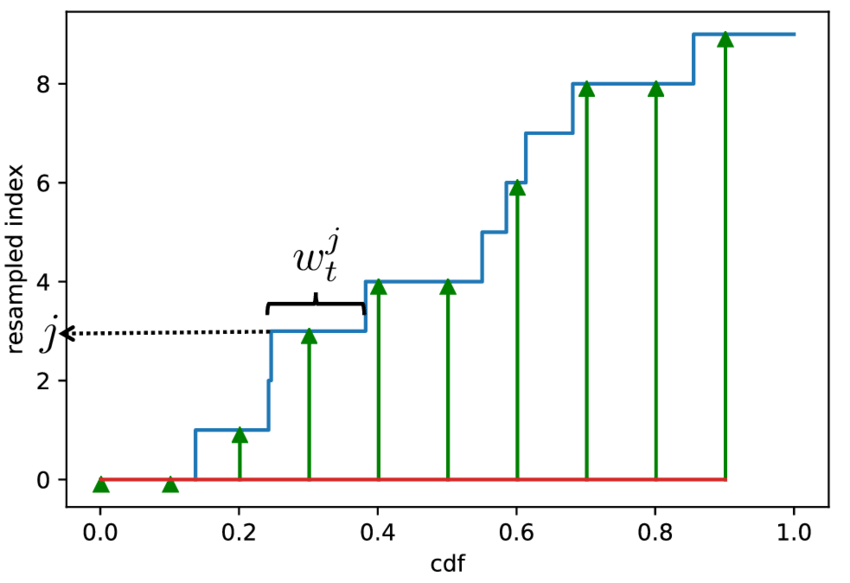
\includegraphics[width=0.9\textwidth]{../../Images/Rééchantillonnage CDF.png}
	\caption{The CDF is defined as the integral of the relevant density function $f$ between $-\infty$ and the current value $x$: $\displaystyle\textup{cdf}:x\mapsto\int_{-\infty}^x{f(t)\:dt}$. In our case, the density is discrete, such that the CDF is piecewise constant, with $\textup{cdf}_0=0$ and $\displaystyle\textup{cdf}_i\triangleq\sum_{j=1}^iw_k^{(j)},\:i\in[\![1,N]\!]$.}\label{fig:CDF}
\end{figure}

\begin{itemize}
	\item\textbf{Multinomial resampling.} All the draws are independent:
	\begin{equation}
		u_j\overset{i.i.d.}{\sim}\mathcal{U}([0,1])
	\end{equation}
	This is the simplest method but has the highest resampling variance.
	\item\textbf{Kitagawa resampling.} A single draw generates all points via:
	\begin{equation}
		\left\{\begin{aligned}
		u_1&\sim\mathcal{U}([0,1/N])\\
		u_j&=u_1+(j-1)/N,\:j\in[\![2,N]\!]
		\end{aligned}\right.
	\end{equation}
	This significantly reduces the variance of the resampling step and is generally preferred in practice.
	\item \textbf{Deterministic resampling.} All draws are deterministic such that, for some $m\in[0,1]$:
	\begin{equation}
		u_j=(j-m)/N,\:j\in[\![1,N]\!]
	\end{equation}
	This eliminates resampling variance entirely at the cost of a deterministic bias.
\end{itemize}

Some advanced filters, such as the auxiliary particle filter, presented in \cref{sec:particle_filtering}, require keeping track of the parent index $i^{(j)}$ of each resampled particle. This value is thus recorded at the creation of each new particle. Using the fact that the CDF and the $u_j$ are increasing, \Cref{alg:Kitagawa} presents the Kitagawa resampling algorithm.

\begin{algorithm}[ht]
	\begin{algorithmic}
	\State{$\textup{cdf}_0=0$}\Comment{Computation of the CDF}
	\State{$\forall i\in[\![1,N]\!],\:\textup{cdf}_i=\textup{cdf}_{i-1}+w_k^{(i)}$\vspace{0.5\baselineskip}}
	\State{$u_1\sim\mathcal{U}([0,1/N])$}\Comment{Kitagawa draws}
	\State{$\forall j\in[\![2,N]\!],\:u_j=u_1+(j-1)/N$\vspace{0.5\baselineskip}}
	\State{$i=1$}
	\For{$j=1:N$}
	\While{$u_j\geq\textup{cdf}_i$}\Comment{Computation of the parent index}
	\State{$i\gets i+1$}
	\EndWhile
	\State{${x^*_k}^{(j)}=x_k^{(i)}$}\Comment{Generation of the new particle}
	\State{${w^*}_k^{(j)}=1/N$}
	\State{$i^{(j)}=i$}
	\EndFor
	\end{algorithmic}\caption{Kitagawa Resampling}\label{alg:Kitagawa}
\end{algorithm}
